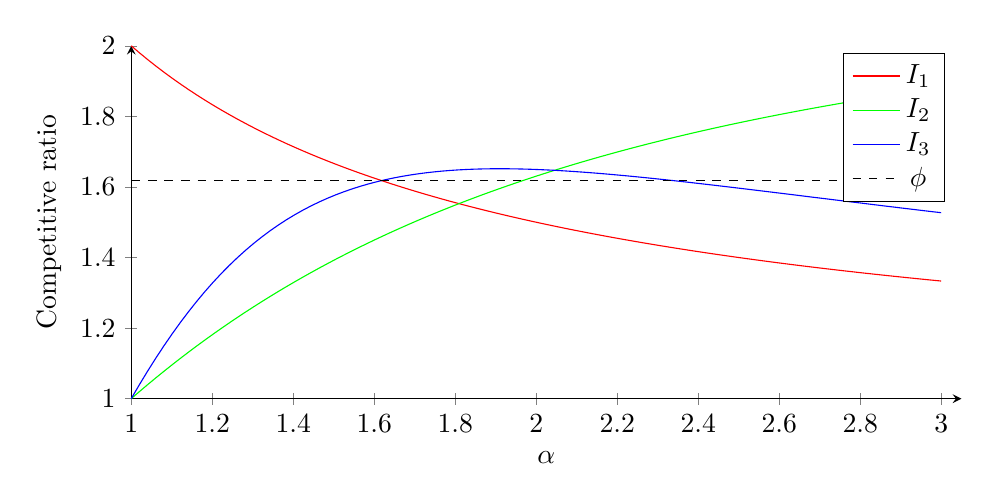
\begin{tikzpicture}
\begin{axis}[
    axis lines = left,
    xmax=3.05,
    xlabel = \(\alpha\),
    ylabel = {Competitive ratio},
    domain=1:3,
    samples=100,
    width=\textwidth,
    height=0.5\textwidth
]
\addplot [
    color=red,
]
{1 + 1/x};
\addlegendentry{\(I_1\)}

\addplot [
    color=green,
]
{(2*x - sqrt(x))/(x - sqrt(x) + 1)};
\addlegendentry{\(I_2\)}

\addplot [
    color=blue,
]
{(2*x^2 - 2 * sqrt(x)^3 + 3*x - 2*sqrt(x))/(2 * x^2 - 2 * sqrt(x)^3 + 1)};
\addlegendentry{\(I_3\)}

\pgfmathsetmacro{\phival}{(1+sqrt(5))/2}

\addplot [
    dashed,
]
{(1 + sqrt(5))/2};
\addlegendentry{\(\phi\)}

\end{axis}
\end{tikzpicture}
